\chapter{Apache Hive}
Hadoop is a popular implementation of the map-reduce model and used widely to process and store extremely large datasets. However, a map-reduce program is very low level and difficult to maintain or reuse. Data scientist come from a world, where SQL is the standard of data processing. Apache Hive gives us a data warehouse solution built on top of Hadoop to write SQL-like queries so we can utilize the advantage of a declarative language. Its language - similar to SQL - is called HiveQL.

\section{Hive \vs RDBMS}
This section shows the main differences between Hive and traditional databases (\eg MySQL, Oracle, MS SQL \etc).

Hive supports SQL interface but it is not a full database. It follows the WORM (Write Once Read Many) model while RDBMS is designed for multiple writes and reads. Hive uses schema on read and traditional databases offer schema on write. Looking into Hive's approach, data is not validated until it is read. We can define multiple schemas on the same data and it provides a fast initial loading since the operation is just a copy and write. However, the schema on read approach has some drawbacks. Schema check on write ensures that the data is not corrupt and it provides a better query performance: when we read data, schema checking is not needed. Hive is a better choice when the schema is not available at loading time since it can be added later dynamically. 

From Hive 0.13, Hive supports transactions \cite{Hive-apache} and full ACID semantics at row level, but with many limitations. Previous to this, atomicity, consistency and durability were available only at partition level. By introducing transactions, Insert, Update and Delete keywords were added to HiveQL. 

The maximum data size allowed in a traditional RDBMS is 10's of Terabytes. However, Hive can easily handle Petabytes.

\subsection{Conclusion}
Hive is a great choice if we want to analyze large, relatively static data sets, fast querying is not necessary and easy, low-cost scalability is required. RDBMS provides fast responses for analyzing data dynamically, but scalability and maximum data size are limited.

\section{Data storage}
Hive structures data in the following units  \cite{Hive-paper, Hive-apache}:
\begin{itemize}
\item \textbf{Databases}: namespaces to avoid conflicts of table, partition or bucket names.
\item \textbf{Tables}: storage unit for data with the same schema. Tables map to directories in HDFS.
\item \textbf{Partitions}: Tables can have multiple partition keys. These will determine how data is stored. In HDFS, partitions map to subdirectories in the table's directory, which speeds up analysis. Instead of running the query in the whole table, Hive will only run our query in the relevant partitions (see example below). Partition columns are virtual, which means they are not part of the data itself.
\item \textbf{Buckets}: Data can be divided into buckets based on the hash value of a column. These help efficiently sample the data. Buckets are stored in files in the table's or partition's directory.
\end{itemize}

\subsection{Example}
This example shows how Hive data units map to HDFS and how partitioning tables can speed up queries.

Hive tables map to \texttt{<warehouse\_root\_directory>/table\_name} directory. The default warehouse root directory is /user/hive/warehouse. This can be changed with the corresponding hive configuration value.
\begin{lstlisting}
	CREATE TABLE test_table(c1 string, c2 int) 
		PARTITIONED BY (date string, hour int);
\end{lstlisting}

The above SQL statement will create a table with two columns and two partitions and it will be stored in  \texttt{/user/hive/warehouse/test\_table} directory in HDFS. Rows with differing date or hour values will be stored in different (separate) partitions. Although the partition columns are not part of the data, they are stored in the table metadata. 

New partitions can be added either with an INSERT or an ALTER statement. These commands will create the corresponding HDFS directories: 
\texttt{/user/hive/warehouse/test\_table/date=2018-01-01/hour=12 and /user/hive/warehouse/test\_table/date=2018-01-02/hour=11}.

\begin{lstlisting}
	INSERT OVERWRITE TABLE
		test_table PARTITION(date='2018-01-01', hour=12)
	SELECT * FROM t;
	
	ALTER TABLE test_table
		ADD PARTITION(date='2018-01-02', hour=11);
\end{lstlisting}

Hive can use this information for pruning the directories to be scanned for query execution. 
\begin{lstlisting}
	SELECT * FROM test_table WHERE date='2018-01-01';
\end{lstlisting}
When executing this query, Hive will only scan the files in \texttt{/user/hive/warehouse/test\_table/date=2018-01-01} directory. Partitioning our data can have a significant impact on the time taken by queries.

Although data in Hive is always in the corresponding directory (\texttt{<warehouse\_root\_directory>/table\_name}), Hive is able to query data stored in other locations in HDFS. In order to do this, we can create EXTERNAL tables thus:
\begin{lstlisting}
	CREATE EXTERNAL TABLE test_external(c1 string, c2 int)
		LOCATION '/user/example_table/example_data';
\end{lstlisting}

Hive assumes that the external table is in its internal format. The difference between an external and default (managed by Hive) table is that the drop table command doesn't affect the data itself in an external table. However, in a managed table, Hive drops the associated data.

\section{Architecture}
The main components of Hive are the following \cite{Hive-paper}:
\begin{itemize}
	\item \textbf{Driver}: manages the lifecycle of a HiveQL query. The Driver also collects the result after the execution phase.
	\item  \textbf{MetaStore}: stores metadata about tables, columns or partitions. For example, it stores the table schema and location.
	\item \textbf{Compiler}: compiles the HiveQL statement and generates the execution plan using the partition and table metadata obtained from the MetaStore. First, it parses the query and does semantic analysis. The Compiler then converts it into AST (Abstract Syntax Tree), and after compatibility checking, to a DAG of Map and Reduce tasks (if Hadoop MapReduce is the execution engine). 
	\item \textbf{Optimizer}: transformations are performed to optimize the DAG for better performance. It is an evolving component. Previously, only rule-based optimization was available which performed column pruning and predicate pushdown. Later, map-side join was introduced and several other join optimizations, as well as cost-based optimization were added.
	\item \textbf{Execution Engine}: executes the plan created by the compiler. The plan is a DAG of stages. The engine manages the dependencies between these stages and executes them in the corresponding component. Hive is compatible with 3 execution engines: MapReduce, Apache TEZ and Spark which can run on Hadoop YARN.
	\item \textbf{HiveServer2}: a service that provides a Thrift interface so clients can execute queries against Hive. Thrift is an RPC (Remote Call Procedure) framework for defining services for multiple languages. HS2 is also the process which contains the Driver.
	\item \textbf{Clients}: multiple clients are available to interact with Hive. Examples include Beeline (CLI), JDBC/ODBC, Python or Ruby client \etc.
\end{itemize}

\begin{figure}[H]
	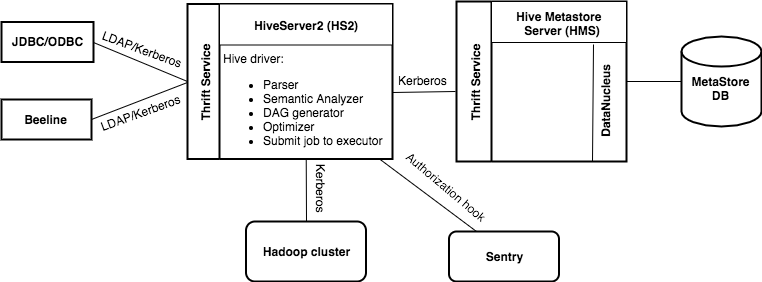
\includegraphics[width=140mm, keepaspectratio]{figures/Hive_architecture.png}
	\centering
	\caption{Hive architecture}
\end{figure}

Clients can connect to HiveServer2 using its Thrift Service. HS2 supports authentication of clients using Kerberos or LDAP authentication. Hive Metastore server also supports Kerberos authentication for Thrift clients.

HMS uses DataNucleus to persist metadata, so many relational databases supported by it can be used: it can be either embedded (\eg Derby) or remote (\eg MySQL) Metastore database.

\section{Life of a Query}
\begin{figure}[H]
	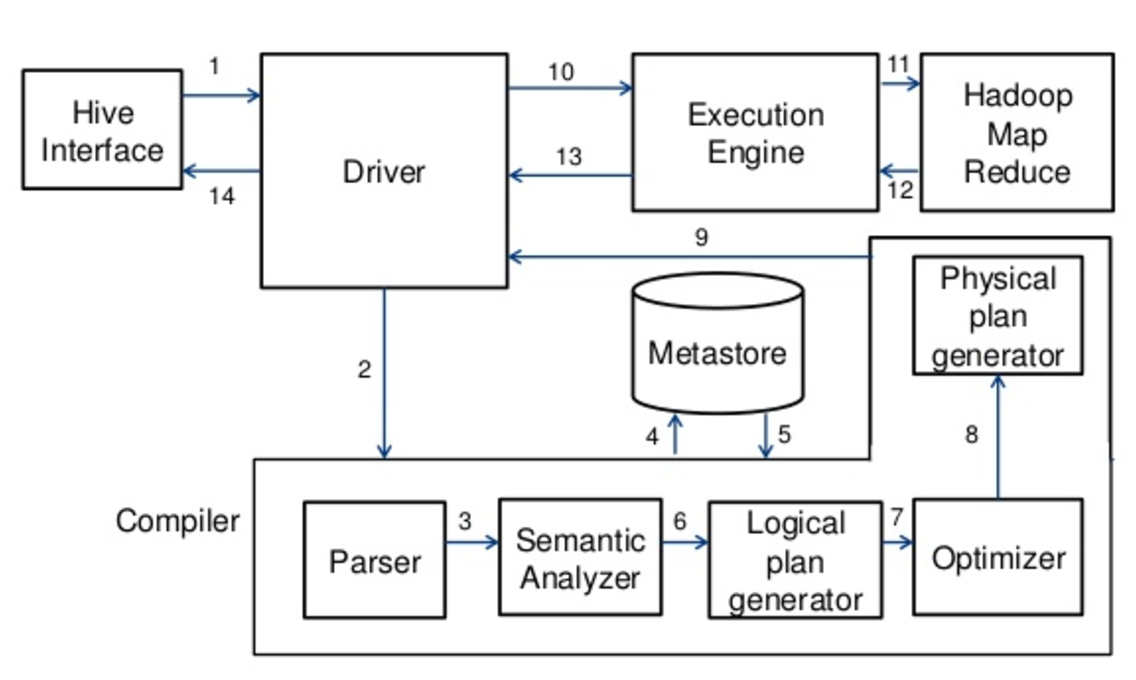
\includegraphics[width=150mm, keepaspectratio]{figures/hive-query.png}
	\centering
	\caption{Life of a query  \cite{Hive-query-figure}}
\end{figure}
The user submits a query using one of the available Hive clients. HiveServer2 recieves the query through its Thrift interface (1). The compilation phase begins:

First, the query is parsed (2), that is transformed into a parse tree using the open source Apache ANTLR.  The semantic analyzer (3) converts the parse tree into a block-based query representation (Query Block Tree). At this phase, connection to Metastore is made (4, 5) to gather information about the tables used by the query, like partition information for later pruning. Type compatibility is checked and semantic errors are flagged.

The logical plan generator (6) transforms the internal representation to an operator tree, which is the logical plan. These operators can either be relational algebra operators (like filter, join) or Hive specific operators (\eg reduceSink) which are later used to convert the query to a series of MapReduce jobs.

Optimization takes place for better performance (7). Some of the optimizations are: 
\begin{itemize}
	\item Column pruning, so only columns needed by the query are kept
	\item Predicate pushdown: this way, the rows can be filtered as soon as possible
	\item Partition pruning: prunes partitions that do not satisfy the predicate
	\item Map-side join: when we join two tables and one of them is small, map-side join can be done. Which means, the small table will be copied to the memory of all the Map nodes.
	\item \etc
\end{itemize}

At physical plan generation (8) the logical plan is split into a series of Map, Reduce tasks (of course if the execution engine is Spark, then to Spark tasks). Also optimization for the specific engine happens at this phase. 

The Driver gets back the physical plan (9) and sends it to the corresponding execution engine (which is MapReduce by default - 10, 11). In this case, Hadoop executes a series of Map and Reduce tasks and returns the result to the Driver (12, 13), which sends it to the user (14).

\section{Hive memory limitations}
HiveServer2 and Hive Metastore require massive resources, especially when it comes to memory. For running up to 40 concurrent queries, the recommended heap size range is 12-16 GB. Once we go above 16 GB it is recommended to split HS2 into multiple instances and load-balance them \cite{Hive-memory-problems}.

Although with a correct configuration and setup we can make our HiveServer2 instance long living, crashes can occur because of Out Of Memory errors (OOM) in certain use-cases. Thus, minimizing the memory footprint whenever we can is a must.

\noindent The memory reserved by HiveServer2 can grow significantly in these situations  \cite{Hive-memory-problems}: 
\begin{itemize}
	\item When we have many table partitions, HS2 needs to load all the partition metadata from HMS. This can cause a significant memory issue, and HiveServer can run out of heap memory and crash.
	\item Concurrent connections can be made to HS2, and memory is directly proportional to the number of connections. 
	\item Complex queries that access a large number of partitions from multiple tables can easily crash HS2.
\end{itemize}

If any of these conditions exist, HS2 can slow down or refuse further connections, queries can fail, and long query compilation or respones retrieval can occur. If the Garbage Collector cannot handle the memory reserved, HiveServer2 can go OOM.
